\documentclass[tocnopagenum]{thesis-ekf}
%a4paper, 12pt, 1.5-es sortávolság, margók
\usepackage[T1]{fontenc}
\PassOptionsToPackage{defaults=hu-min}{magyar.ldf}
\usepackage[magyar]{babel}
\usepackage{mathtools,amssymb,amsthm,pdfpages}
\footnotestyle{rule=fourth}
\usepackage{comment}
\usepackage{enumitem}
\usepackage{colortbl}
\newtheorem{tetel}{Tétel}[chapter]
\theoremstyle{definition}
\newtheorem{definicio}[tetel]{Definíció}
\theoremstyle{remark}
\newtheorem{megjegyzes}[tetel]{Megjegyzés}
\graphicspath{{./images/}}
\DeclareGraphicsExtensions{.png,.jpg,.pdf}
%excel to latex
\usepackage{booktabs}
\usepackage{bigstrut}


\begin{document}
	\institute{Matematikai és Informatikai Intézet}
	\title{Informatikai eszközökkel támogatott sport és egészségfejlesztés}
	\author{Sipos Levente\\Szak: Programtervező informatikus BSc\\Specializáció: Szoftverfejlesztő informatikus}
	\supervisor{Dr. Király Roland\\docens}
	\city{Eger}
	\date{2022}
	\begin{titlepage}
		\maketitle
	\end{titlepage}
	
	\tableofcontents

	\addcontentsline{toc}{chapter}{Bevezetés}
	\addcontentsline{toc}{chapter}{Elméleti háttér}
	\addcontentsline{toc}{chapter}{Összegzés}



	\begin{comment}
		leírom hogy miről szól, (nem kötelező), 2 rész -> probléma felvetés, mi a motiváció, kontextus, előremutatva a dolgozatban hol miről fogsz beszélni.(1.fejezetben befogom mutatni a kódolást)
	\end{comment}
	\chapter*{Bevezetés}
	A tanulmányaim során sok olyan tárgyat tanulhattam amelyek segítettek belátást nyerni, hogy valójában melyik is az az irányágazat az informatikán belül, amely felkeltette az érdeklődésemet. Az utolsó félévekben tanulhattam robotikát a Robotika alapjai nevezetű tárgy következtében, amely közelebb vitt engem a gépközeli programozás világába. Továbbá C\# nyelvben elég biztos tudást szerezhettem a Szolgáltatás Orientált Programozás, Magasszintű programozási nyelvek I. és II. című tárgyakon.
	\par
	Szakdolgozatom tematikájául szerettem volna egy olyan témát választani, melynek a későbbiekben másoknak tudok segítséget nyújtani az informatikai szaktudásommal.
	Mint keresztény hívő ember, úgy gondolom, hogy az emberi létünk egyik fő feladat és mozgatórúgója az az, hogy segítsünk embertársainkon azokkal a technikákkal és tudásokkal amelyek számunkra megadattak. Ezért örömmel tölt el az a lehetőség, hogy tanulmányaimat ennek a segítségére fordíthatom. 
	\par
	A választott téma, mind az informatika mind, az egészségügy számára fontos kérdéseket tehet fel:
	\begin{itemize}
		\item  Mi jelenthet arra megoldást, ha egy adott korosztályba tartozó ember, nehézségekkel küzd a mindennapokban, a mozgását, illetve a mentális felfogását illetően? (Akár ez jelentheti az egyszerű mozgások nem megfelelő elvégzését, akár pedig az alap információk felfogásában való akadályozottságot is.)
		\item  Az informatikával tudunk-e az előbb említett kérdésre, olyan alkalmazást írni, amely ezeknek a fejlődését elősegítheti?
		\item A testnevelés tudomány és a technika az informatikával társítva, hogyan tudja segíteni az emberi mozgást?
		\item Amennyiben tudunk ilyen alkalmazást írni, hogyan valósítsuk meg?
	
	\end{itemize}
 	Ezen kérdések alapján keresem a válaszokat arra nézve, hogy az informatika hogyan tud segítségére lenni a fizikai létnek. 
 
	Meglátásom szerint, ez egy hiánypótló kutatási téma, amely az embereknek a mozgását, és fizikai jólétét segítheti elő.
	Ezen eszközök leptikus területeket érintenek, vizuális illetve akusztikus hatások közreműködésével.
	\\
	A projekt fontossága az, hogy ezen eszközök segítséget tudjanak nyújtani, esetleg kiváltsák a beszédnek a szolgálatát. Ahol már beszéd nem elegendő ott ezen eszközök segíthetik a mozgásában fejlődésre szoruló egyéneket. Mind a fiatalok mind a szépkorúak számára hasznos gyakorlat lehet.
	\\ 
	A digitális fejlődéssel egyre több eszköz segíti az arra rászorulókat, például a mostanság kutatásban lévő gondosóra, program amely a szociális segítésben vesz részt az idősgondozásban.\cite{MTI}
	\\
	A cél az embereknek a fizikai illetve mentális állapotának elősegítése.
	\par 
	
	Alapvetően a következő fejezetekben azt szeretném részletezni, hogy milyen technológiákat használunk, és emellett milyen programozási nyelven készül a projekt. \\ 
	Továbbá, ki fogok térni azokra a rendszerekre is, amelyek hasonló céllal készültek el. Majd ezen projekteket hasonlóságait és különbségeit mérném össze, az elkészült projektünkkel. 
	
	\begin{comment}
	Bevezető2: Rendszer amit kidolgozott Somodi László, mi a szerepe, mi a célja, mit vállaltam én? -> frontend
	\end{comment}
	\chapter*{Bevezető 2}
	\par
	A témában jártas, és a "Mozgáskoordináció- és gyorsaságfejlesztő gyakorlatok óvodától a felnőtt korig" \cite{SLaszlo} című könyv írója, Somodi László, segített belátást nyerni az egészségügyi és a morális lényegességébe a projektnek. \\ Elmondása szerint a mozgásfejlesztés és az agyi kapacitás fejlesztése, kéz a kézben jár. Ezt a mozgásfejlesztést úgy érhetjük el, ha az adott személynek utasításokat adunk ki, hogy adott jelzésre (szín, hang, irány) és ezek kombinációjára, milyen mozgást kell végeznie.
	\par 
	\subsection*{Gyakorlati haszna}
	Az agy mentális funkcióinak erősítése, speciális koordinációfejlesztő gyakorlatokkal is lehetséges melynek a három komponense a következő: 
	\begin{enumerate}
	 
			\item	Az első komponens a koncepció, vagyis az a módszer, ami alapján a rendszer elkészült. A koncepció egészségügyi, és sport-rekreációs tevékenység alapú.
			\item	A második komponens a hardver, ami a mozgáshoz és a gyakorláshoz szükséges időzítést, jelzéseket adja, és vezérli az aktivitást, amit a koncepció előír.
			\item	A harmadik komponens a hardvert meghajtó, és így a feladatokat közvetlenül irányító, programozható, tanítható szoftver.
	\end{enumerate}
	\subsection*{Módszer lényege}
	Az a személy aki használja ezt, nála külön dolgozik a két kar, külön dolgozik a két láb és ezáltal folyamatosan kapcsoljuk át a két agyféltekét.
	Továbbá, a könnyen és egyszerűen felismerhető hang, szín, és ábra jelzések az esetlegesen a fogyatékossággal élő emberek számára se jelenthet akadályt.
	\\
	Különféle álló helyzetek (alapállás, mellső középtartás, magas tartás) képesek segíteni abban, hogy az idegpályákon lévő átkapcsolódási pontok (szinapszisok) száma növekedjen. Fiatalabb korban a szinapszisok számát, későbbiekben az átkapcsolódási pontok erejét növeli.
	Sokféle betegség felmerülhet az olyan embereknél akiknek ez a módszer alkalmas lehet, a könnyen felismerhető és megérthető eszközök.
	Továbbá, ez által a módszer által gyorsabban megértjük az elvégzendő  feladatot, feladatokat és akár gyorsabban is végrehajthatjuk azokat.
	  %szellemi leépüléssel küzdő, szép korúak számára is segítséget nyújthat, mivel a változatos mozgás, és a különböző ingerek ki- és be- kapcsolása növeli az agy alap működését.
	 \\
	Gyakorlati tapasztalatunk szerint a módszer hasznosan alkalmazható általános helyzetű, HH és HHH helyzetű és beteg gyerekeknél is. Kutatásaink és mért eredményeink ezt támasztják alá.
	A módszert kis helyen és minden korosztálynál lehet alkalmazni, de a teljesség érdekében, a módszer intelligens szobával együtt működik hatékonyan.
	
	
	\subsection*{Intelligens szoba röviden}
	Az intelligens szoba kifejezés egy olyan helység, melynek mind a négy falán, vagy oldalán különböző jeladókat helyezünk el.
	Ezek különböző eszközök melyek típusai lehetnek: fények, színek, nyilak és hangok. Ezek külön, vagy együttesen kiküldött jeleire különböző, illetve speciális koordinációfejlesztő feladatokat végrehajtani. Minden egyes különböző szín, és fényjelzés, más és más feladatokat tartalmaznak.
	Ez azt jelenti, hogy adott esetben egy piros lámpa színe emlékeztethet arra, hogy a piros szín jelentése szimbolikus hatással bír.Melyet az adott ember köthet a már mindennapos életben tapasztaltakhoz. Nyilak felvillanására, különböző hangokra pedig más érzékeket váltunk ki mint például a fényjelzés esetén. Ilyenkor irányváltásokat kell végrehajtani amik máris komplikálják egy kicsit az adott mozdulatokat.
	\\
	Ezzel a módszerrel és az intelligens szobával együttesen tudjuk a mozgáson keresztül úgy stimulálni az agyat, hogy a legrövidebb idő alatt a legtöbbször átkapcsoljuk. ( 200-szor, 300-szor, 400-szor, stb. )
	\par
	\subsection*{Automatizálás célja}
	A fentebb említettek automatizálására készül a projekt, amely különböző informatikai eszközökkel valósítja meg a színek, hangok, és nyilak megjelenítését, illetve érzékeltetését. 
	A hardver komponensek. A hardver több egymáshoz tetszőlegesen kapcsolható smart box, amelyek képesek fényjelzések, fénnyel képzett ábrák, valamint hangjelzések kiadására. A smart box-okat szoftveresen lehet vezérelni, így azok képesek a koncepció alapján összetett mozgások, vagy komplex feladatsorok irányítására.
	Ennek egy példája a \pageref{table:egyedzesterv}. oldalon található táblázat amely az automatizálásra létrehozott "edzéstervet" mutat be.[\ref{table:egyedzesterv}]
	\begin{table}[h]
		\centering
		\caption{Egy adott edzésterv}
		\scalebox{0.7}
		{
			\begin{tabular}{|rrrrlrrrrr|}
				\hline
				\multicolumn{1}{|l|}{\textbf{helyzet}} & \multicolumn{1}{l|}{\textbf{egység típusa}} & \multicolumn{1}{l|}{\textbf{jel száma}} & \multicolumn{1}{l|}{\textbf{szín}} & \multicolumn{1}{l|}{\textbf{hang}} & \multicolumn{1}{l|}{\textbf{irány}} &       &       & \multicolumn{1}{l}{\textbf{fenntartási idő}} & \multicolumn{1}{l|}{\textbf{irány}} \bigstrut\\
				\hline
				&       &       &       &       &       &       &       &       &  \bigstrut[t]\\
				&       &       &       &       &       &       &       &       &  \\
				\multicolumn{1}{|c}{1} & \multicolumn{1}{c}{2} & \multicolumn{1}{c}{3} & \multicolumn{1}{c}{4} & \multicolumn{1}{c}{5} & \multicolumn{1}{c}{6} & \multicolumn{1}{c}{7} & \multicolumn{1}{c}{8} &       &  \\
				\multicolumn{1}{|c}{lámpa} & \multicolumn{1}{c}{lámpa} & \multicolumn{1}{c}{hang} & \multicolumn{1}{c}{lámpa} & \multicolumn{1}{c}{nyíl} & \multicolumn{1}{c}{lámpa} & \multicolumn{1}{c}{lámpa} & \multicolumn{1}{c}{nyíl} &       &  \\
				&       &       &       &       &       &       &       &       &  \\
				\multicolumn{1}{|l}{szemben} &       &       &       &       &       &       &       &       &  \bigstrut[b]\\
				\cline{1-2}\cline{7-7}    \rowcolor[rgb]{ .6,  .8,  0} \multicolumn{1}{|c|}{\textcolor[rgb]{ .2,  .6,  .4}{zöld}} & \multicolumn{1}{c|}{\cellcolor[rgb]{ 1,  0,  0}piros} & \cellcolor[rgb]{ 1,  1,  1} & \multicolumn{1}{c}{\cellcolor[rgb]{ 1,  1,  0}sárga} & \cellcolor[rgb]{ 1,  1,  1} & \multicolumn{1}{c|}{\cellcolor[rgb]{ .2,  .4,  1}kék} & \multicolumn{1}{l|}{\cellcolor[rgb]{ 1,  1,  1}fehér} & \cellcolor[rgb]{ 1,  1,  1} & \cellcolor[rgb]{ 1,  1,  1} & \cellcolor[rgb]{ 1,  1,  1} \bigstrut\\
				\cline{1-2}\cline{7-7}    \rowcolor[rgb]{ 0,  0,  0}       &       &       &       &       &       &       &       &       &  \bigstrut\\
				\cline{2-2}    \multicolumn{1}{|r|}{} & \multicolumn{1}{c|}{\cellcolor[rgb]{ 1,  0,  0}1 piros} &       &       &       &       &       &       & \multicolumn{1}{c}{16"} &  \bigstrut\\
				\cline{2-2}\cline{4-4}          &       & \multicolumn{1}{c|}{} & \multicolumn{1}{c|}{\cellcolor[rgb]{ 1,  1,  0}2 sárga} &       &       &       &       & \multicolumn{1}{c}{1"} &  \bigstrut[t]\\
				&       & \multicolumn{1}{c|}{} & \multicolumn{1}{c|}{\cellcolor[rgb]{ 1,  1,  0}2 sárga} &       &       &       &       & \multicolumn{1}{c}{16"} &  \bigstrut[b]\\
				\cline{1-1}\cline{4-4}    \rowcolor[rgb]{ .6,  .8,  0} \multicolumn{1}{|c|}{1 zöld} & \cellcolor[rgb]{ 1,  1,  1} & \cellcolor[rgb]{ 1,  1,  1} & \cellcolor[rgb]{ 1,  1,  1} & \cellcolor[rgb]{ 1,  1,  1} & \cellcolor[rgb]{ 1,  1,  1} & \cellcolor[rgb]{ 1,  1,  1} & \cellcolor[rgb]{ 1,  1,  1} & \multicolumn{1}{c}{\cellcolor[rgb]{ 1,  1,  1}1"} & \cellcolor[rgb]{ 1,  1,  1} \bigstrut[t]\\
				\rowcolor[rgb]{ .6,  .8,  0} \multicolumn{1}{|c|}{1 zöld} & \cellcolor[rgb]{ 1,  1,  1} & \cellcolor[rgb]{ 1,  1,  1} & \cellcolor[rgb]{ 1,  1,  1} & \cellcolor[rgb]{ 1,  1,  1} & \cellcolor[rgb]{ 1,  1,  1} & \cellcolor[rgb]{ 1,  1,  1} & \cellcolor[rgb]{ 1,  1,  1} & \multicolumn{1}{c}{\cellcolor[rgb]{ 1,  1,  1}16"} & \cellcolor[rgb]{ 1,  1,  1} \bigstrut[b]\\
				\cline{1-1}\cline{6-6}          &       &       &       & \multicolumn{1}{c|}{} & \multicolumn{1}{c|}{\cellcolor[rgb]{ .2,  .4,  1}1 kék} &       &       & \multicolumn{1}{c}{1"} &  \bigstrut[t]\\
				&       &       &       & \multicolumn{1}{c|}{} & \multicolumn{1}{c|}{\cellcolor[rgb]{ .2,  .4,  1}1 kék} &       &       & \multicolumn{1}{c}{8"} &  \bigstrut[b]\\
				\cline{4-4}\cline{6-6}          &       & \multicolumn{1}{r|}{} & \multicolumn{1}{c|}{\cellcolor[rgb]{ 1,  1,  0}2 sárga} &       &       &       &       & \multicolumn{1}{c}{1"} &  \bigstrut[t]\\
				&       & \multicolumn{1}{r|}{} & \multicolumn{1}{c|}{\cellcolor[rgb]{ 1,  1,  0}2 sárga} &       &       &       &       & \multicolumn{1}{c}{16"} &  \bigstrut[b]\\
				\cline{4-4}\cline{7-7}          &       &       &       &       & \multicolumn{1}{r|}{} & \multicolumn{1}{c|}{1 fehér} &       & \multicolumn{1}{c}{1"} &  \bigstrut[t]\\
				&       &       &       &       & \multicolumn{1}{r|}{} & \multicolumn{1}{c|}{1 fehér} &       & \multicolumn{1}{c}{4"} &  \bigstrut[b]\\
				\cline{3-3}\cline{7-7}          & \multicolumn{1}{r|}{} & \multicolumn{1}{l|}{3 - 1 bip} &       &       &       &       &       &       & \multicolumn{1}{l|}{ford. jobbra} \bigstrut\\
				\cline{3-3}    \rowcolor[rgb]{ 0,  0,  0}       &       &       &       &       &       &       &       &       &  \bigstrut[t]\\
				& \multicolumn{1}{c}{\cellcolor[rgb]{ 1,  0,  0}4 piros} &       &       &       &       &       &       & \multicolumn{1}{c}{8"} &  \\
				\rowcolor[rgb]{ .6,  .8,  0} \multicolumn{1}{|c}{5 zöld} & \cellcolor[rgb]{ 1,  1,  1} & \cellcolor[rgb]{ 1,  1,  1} & \cellcolor[rgb]{ 1,  1,  1} & \cellcolor[rgb]{ 1,  1,  1} & \cellcolor[rgb]{ 1,  1,  1} & \cellcolor[rgb]{ 1,  1,  1} & \cellcolor[rgb]{ 1,  1,  1} & \multicolumn{1}{c}{\cellcolor[rgb]{ 1,  1,  1}1"} & \cellcolor[rgb]{ 1,  1,  1} \\
				\rowcolor[rgb]{ .6,  .8,  0} \multicolumn{1}{|c}{5 zöld} & \cellcolor[rgb]{ 1,  1,  1} & \cellcolor[rgb]{ 1,  1,  1} & \cellcolor[rgb]{ 1,  1,  1} & \cellcolor[rgb]{ 1,  1,  1} & \cellcolor[rgb]{ 1,  1,  1} & \cellcolor[rgb]{ 1,  1,  1} & \cellcolor[rgb]{ 1,  1,  1} & \multicolumn{1}{c}{\cellcolor[rgb]{ 1,  1,  1}8"} & \cellcolor[rgb]{ 1,  1,  1} \\
				&       &       &       &       &       & \multicolumn{1}{l}{4 fehér} &       & \multicolumn{1}{c}{1"} &  \\
				&       &       &       &       &       & \multicolumn{1}{l}{4 fehér} &       & \multicolumn{1}{c}{8"} &  \\
				&       &       & \multicolumn{1}{c}{\cellcolor[rgb]{ 1,  1,  0}4 sárga} &       &       &       &       & \multicolumn{1}{c}{1"} &  \\
				&       &       & \multicolumn{1}{c}{\cellcolor[rgb]{ 1,  1,  0}4 sárga} &       &       &       &       & \multicolumn{1}{c}{8"} &  \\
				&       & \multicolumn{1}{l}{hang semleges} &       &       &       &       &       & \multicolumn{1}{c}{1"} &  \\
				&       & \multicolumn{1}{l}{hang semleges} &       &       &       &       &       & \multicolumn{1}{c}{8"} &  \\
				&       &       &       & zöld nyíl &       &       &       &       &  \bigstrut[b]\\
				\hline
			\end{tabular}%
		}
		\label{table:egyedzesterv}%
	\end{table}%
	
	\begin{comment}
		Itt még lehetne kicsit beszélni a Somodi Lászlós dologokról.
	\end{comment}

	Alapvetően, a projekten sok személy részt vett, a hardver lefejlesztésében és 
	összeszerelésében, Keresztes Péter Tanár úr. \\
	A back-end és ezeknek a hardvereknek a mögöttes működtetését, valamint a Delphi és a C\# nyelvek közötti kapcsolat megoldását, Nagy-Tóth Bence, barátom és szaktársam készítette el.
	\\
	Én ezeknek a hardvereknek a működtetéséhez a felületet írtam, amin keresztül lehet különféle módon, változatos ütemekben vezérelni a fentebb említett eszközöket. Ezt C\# nyelven írtam ami a felhasználói felület írására kellően alkalmas.
	
	
	\begin{comment}
		1.fejezet: Milyen technológiákat használunk, milyen nyelv, architektúrák, kapcsolási rajz, interface, ui, meg ezek hogyan néznek ki.
	\end{comment}
	\chapter*{1.fejezet}
	\subsection{C\# fejlődése}
	A szakdolgozatom projektje C\# nyelven íródik amely a legjobban alkalmazkodik az ilyen felületek leimplementálásához. \\
	A C\# nyelv alapvetően a Microsoft által kifejlesztett objektumorientált programozási nyelv.
	Ezentúl ez egy egyszerű, modern programozási nyelv amely egybeköti a C és a C++ nyelv erejét az új applikáció fejlesztésével egybekötve. \cite{hejlsberg2003c}
	\\ 
	Számos főbb újdonságokat implementáltak ebbe a nyelvbe, megemlítésre méltóak például a 2005-ös verzióban létrejövő Generikus és parciális típusok amelyek megkönnyítették a programozó munkáját, mivel általánosabb kódot tudtak írni ezek segítségével.
	Ezentúl, még hasonlóságokat is fedezhetünk fel például a Java nyelvben, amely egyezést mutat számos helyen.
	Mint például az osztályok deklarálása, metódusok illetve függvények létrehozása. Emellett a mezők szintaxisa is megegyező.
	\\
	A C\#-ban még sok más opciónk is van programok fejlesztésére, ilyen például a Konzolos Applikáció(Console Application), a Windows Forms Application, illetve a WPF(Windows Presentation Foundation). Ezen utóbbi kettő applikáció segítségével ablakos illetve asztali alkalmazásokat készíthetünk.
	\\
	A projektem során azért választottam a Windows Forms Application-t mivel a különböző eszközök(gombok, címkék) amelyek az ezen alkalmazásban megtalálhatóak elősegítik a felhasználó számára a könnyed olvashatóságot és feltérképezés lehetőségét. Az alkalmazás hasonló módon elkészülhetett volna konzolos felületre is, de mivel ez a felhasználó és az esetlegesen laikus ügyfél számára is nehezen érthető, ezért az ablakos alkalmazás a támogatott.
	\\ 
	\subsection*{DLL}
	C\#-ban lehetőség van úgynevezett DLL-ek használatára is. A DLL(Dynamic Link Library) mint olyan az egy kisebb programok összessége, amelyeket nagyobb programok könnyűszerrel be tudnak importálni a saját projektjükbe. Ezen kisebb programokhoz vagy DLL fájlokhoz, hozzátartozik leírás is amelyek általában minden egyes függvényeknél, illetve metódusoknál megjegyezhető. Ennek oka, hogy az a fejlesztő aki használja a DLL-t
	nagyobb belátást kapjon arról hogy az adott metódus, miként és hogyan működik.
	\\
	A projekthez a DLL-t, Nagy-Tóth Bence hallgatótársam szolgáltatja amelyben számos metódus meg lett írva, ezeket felhasználva a fő applikáció működésre bírható.
	\\
	Ezentúl, a működtettet eszközökkel való kommunikációt Delphi programozási nyelvben volt szükséges megírni amely a DLL alapját képezte. 
	\\
	\subsection*{eszközök}
	Háromféle eszközt működtetünk, lámpát, nyilakat szimbolizáló lámpa, illetve egy hangszóró.
	Ezen eszközöknek önálló tápellátással rendelkeznek, melyek közötti kapcsolatot 4 pólusú RJ típusú csatlakozókkal felszerelt kábelen keresztül lehet biztosítani. Az egyes egységeket láncszerűen kell egymás után kapcsolni, melyeket vagy individuálisan vagy kollektívan lehet kötni a vezérlő számítógéphez. Ezen összekötéshez szükséges egy USB 2.0-ás nyomtatókábel, melynek az USB-B-s fele az eszközbe csatlakozik, és az USB-A-s fele pedig a tápot biztosító és programot futtató számítógépbe.
	\\  
	A hangszóró adott hangszínt le tud játszani, amelyeket különbőző hosszúságig illetve hangerősségbe tudunk működtetni.
	Az ehhez tartozó kapcsolási rajzok megtalálhatóak a [\ref{fig:hangsz1}],[\ref{fig:hangsz2}],[\ref{fig:hangsz3}] ábrák alatt.
	\par
	A lámpa egy olyan eszköz lesz amelyen különböző színben tud világítani a LED, különböző időközönként. Természetesen a világítás hosszát is be lehet állítani különböző eszközökhöz.
	Az ehhez tartozó kapcsolási rajzot a [\ref{fig:lamp1}],[\ref{fig:lamp2}],[\ref{fig:lamp3}] ábrák alatt.
	\par
	A nyíl egy olyan eszköz lesz amelyen különböző színben tud világítani a LED-ek összessége, illetve különböző irányba tud mutatni a LED-ek által kialakított alakzat.  Természetesen  világítás hosszát is be lehet állítani különböző eszközökhöz, különböző időközönként.
Az ehhez tartozó kapcsolási rajzot a [\ref{fig:nyil1}],[\ref{fig:nyil2}],[\ref{fig:nyil3}] ábrák alatt.\medskip
\\
	%Hangszóró:
	\begin{figure}[h!]
	
	\centering
	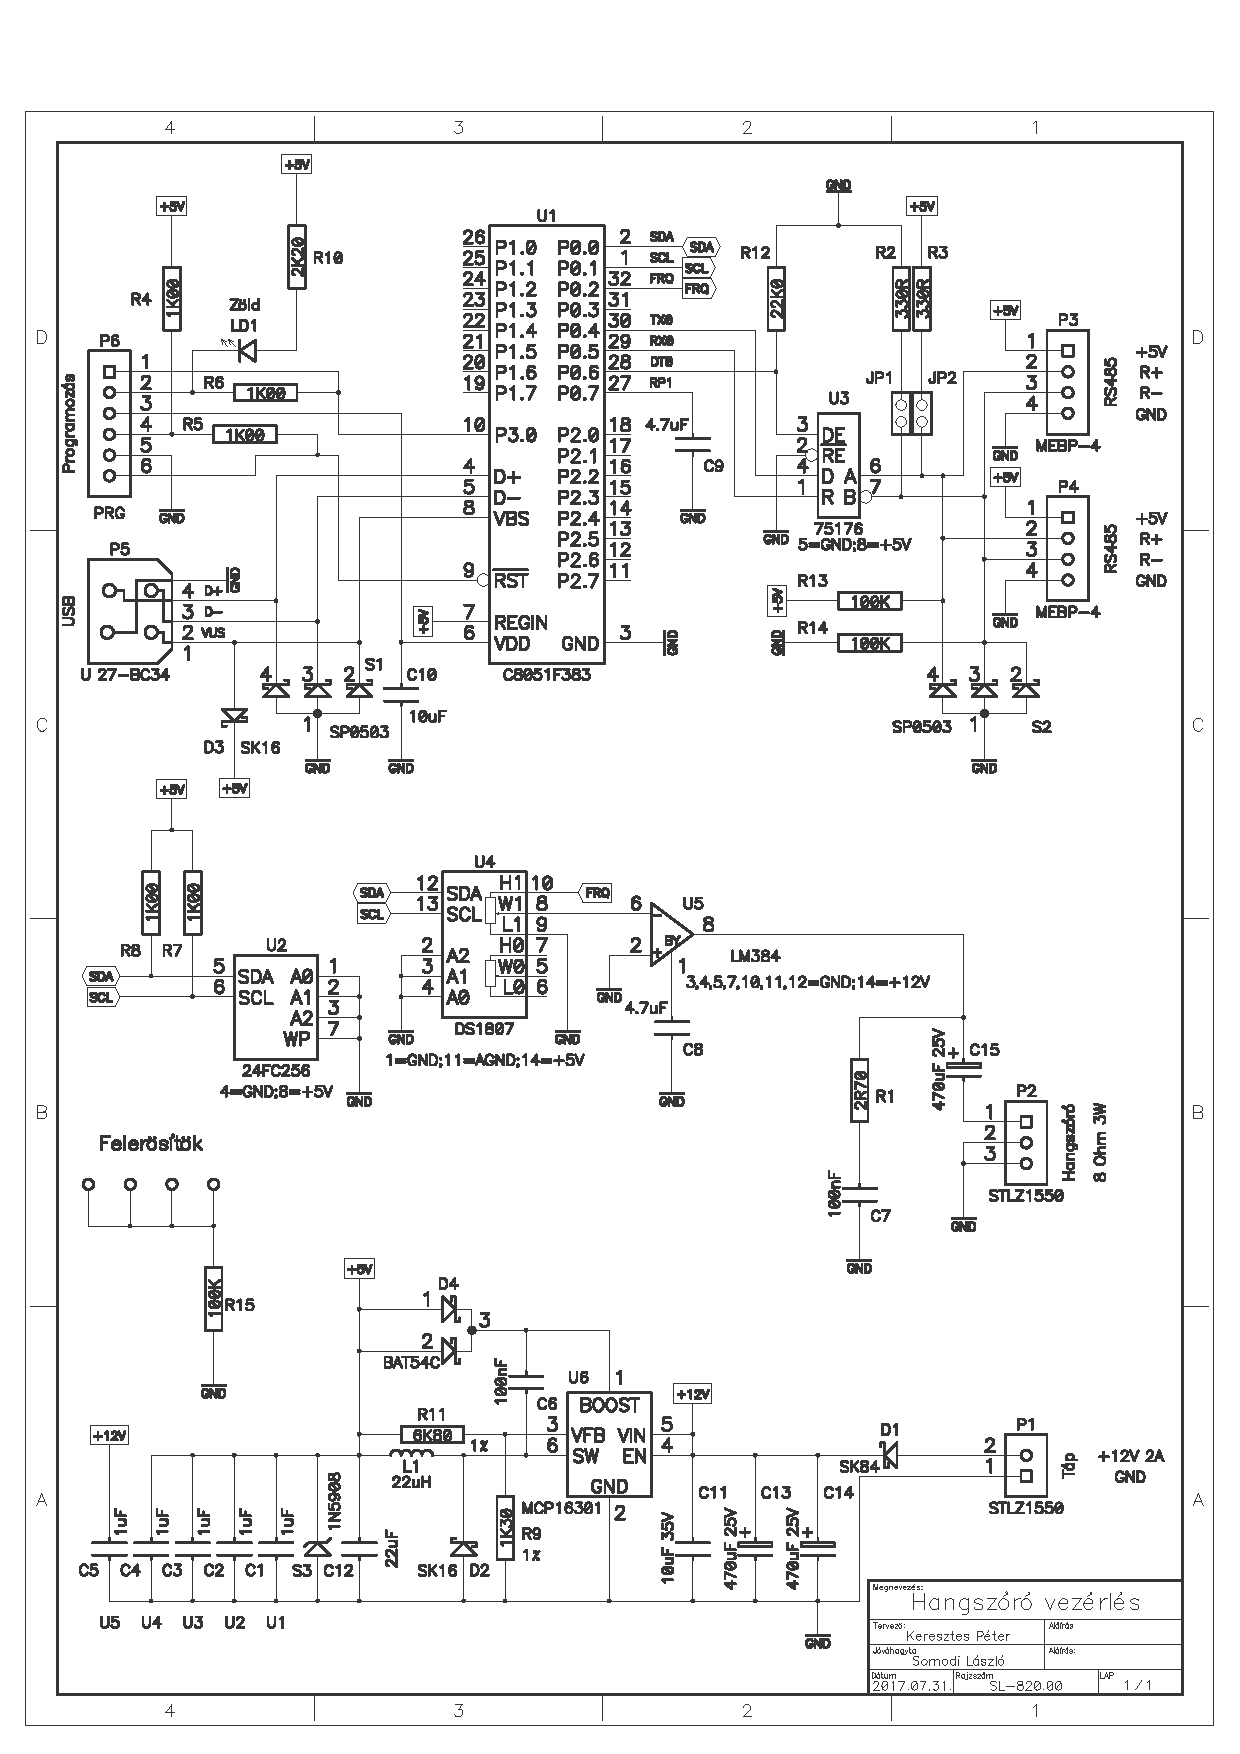
\includegraphics[page=1,width=0.5\textwidth]{SLH}
	\caption{hangszóró kapcsolási rajz \#1}
	\label{fig:hangsz1}
	
	\end{figure}
	\begin{figure}[h!]
		\centering
		\includegraphics[page=2,width=0.5\textwidth]{SLH}
		
		\caption{hangszóró kapcsolási rajz \#2}
		\label{fig:hangsz2}
	\end{figure}
	\begin{figure}[h!]
	
		\centering
		\includegraphics[page=3,width=0.5\textwidth]{SLH}
		
		\caption{hangszóró kapcsolási rajz \#3}
		\label{fig:hangsz3}\medskip
	\end{figure} 


	%lámpa
	\begin{figure}[t]
	
		\centering
		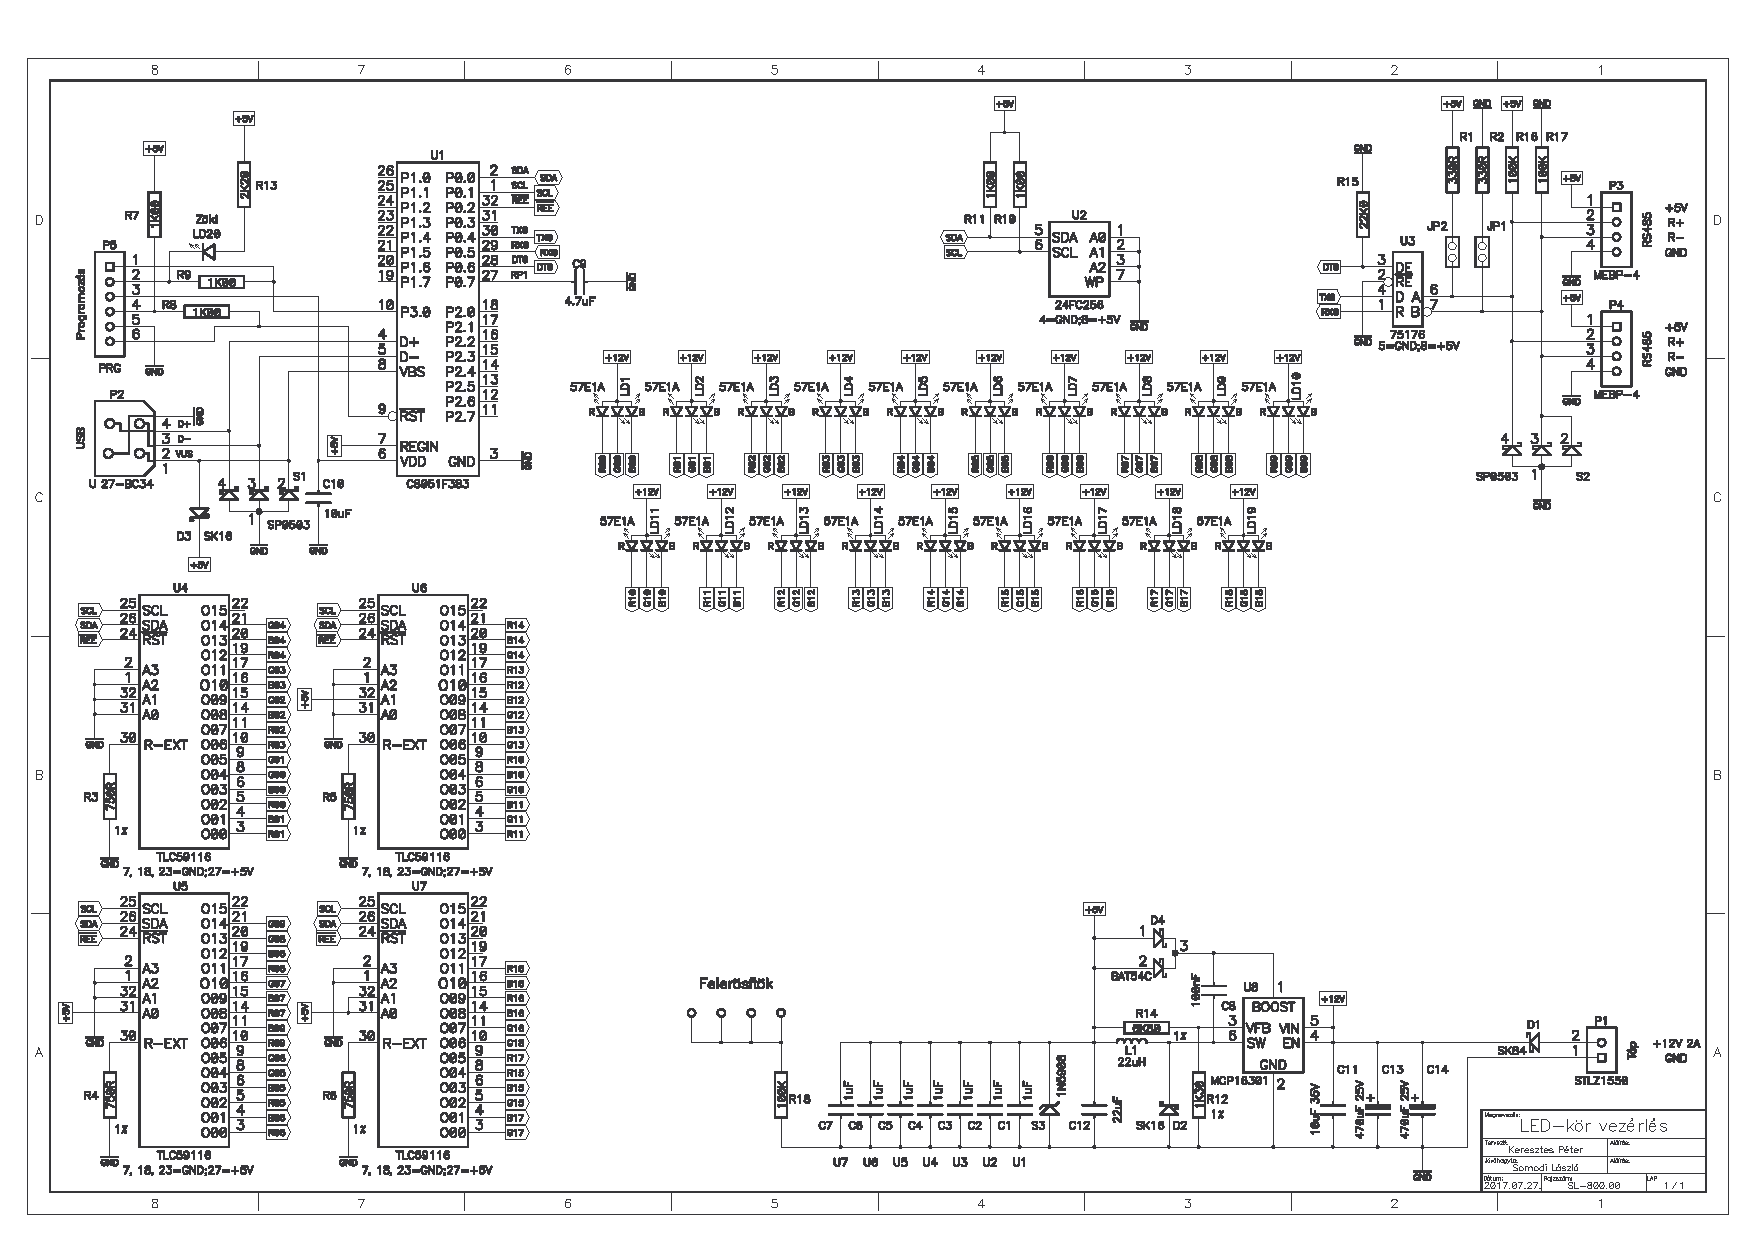
\includegraphics[page=1,width=0.5\textwidth]{SLL}
		
		\caption{lámpa kapcsolási rajz \#1}
			\label{fig:lamp1}
	
	\end{figure}
	\begin{figure}[t]
	
		\centering
		\includegraphics[page=2,width=0.5\textwidth]{SLL}
		
		\caption{lámpa kapcsolási rajz \#2}
		\label{fig:lamp2}
	
	\end{figure}
	\begin{figure}[t]
		
		\centering
		\includegraphics[page=3,width=0.5\textwidth]{SLL}
		
		\caption{lámpa kapcsolási rajz \#3}
		\label{fig:lamp3}
	
	\end{figure}
\par


	%nyíl
	\begin{figure}[h]
		\centering
		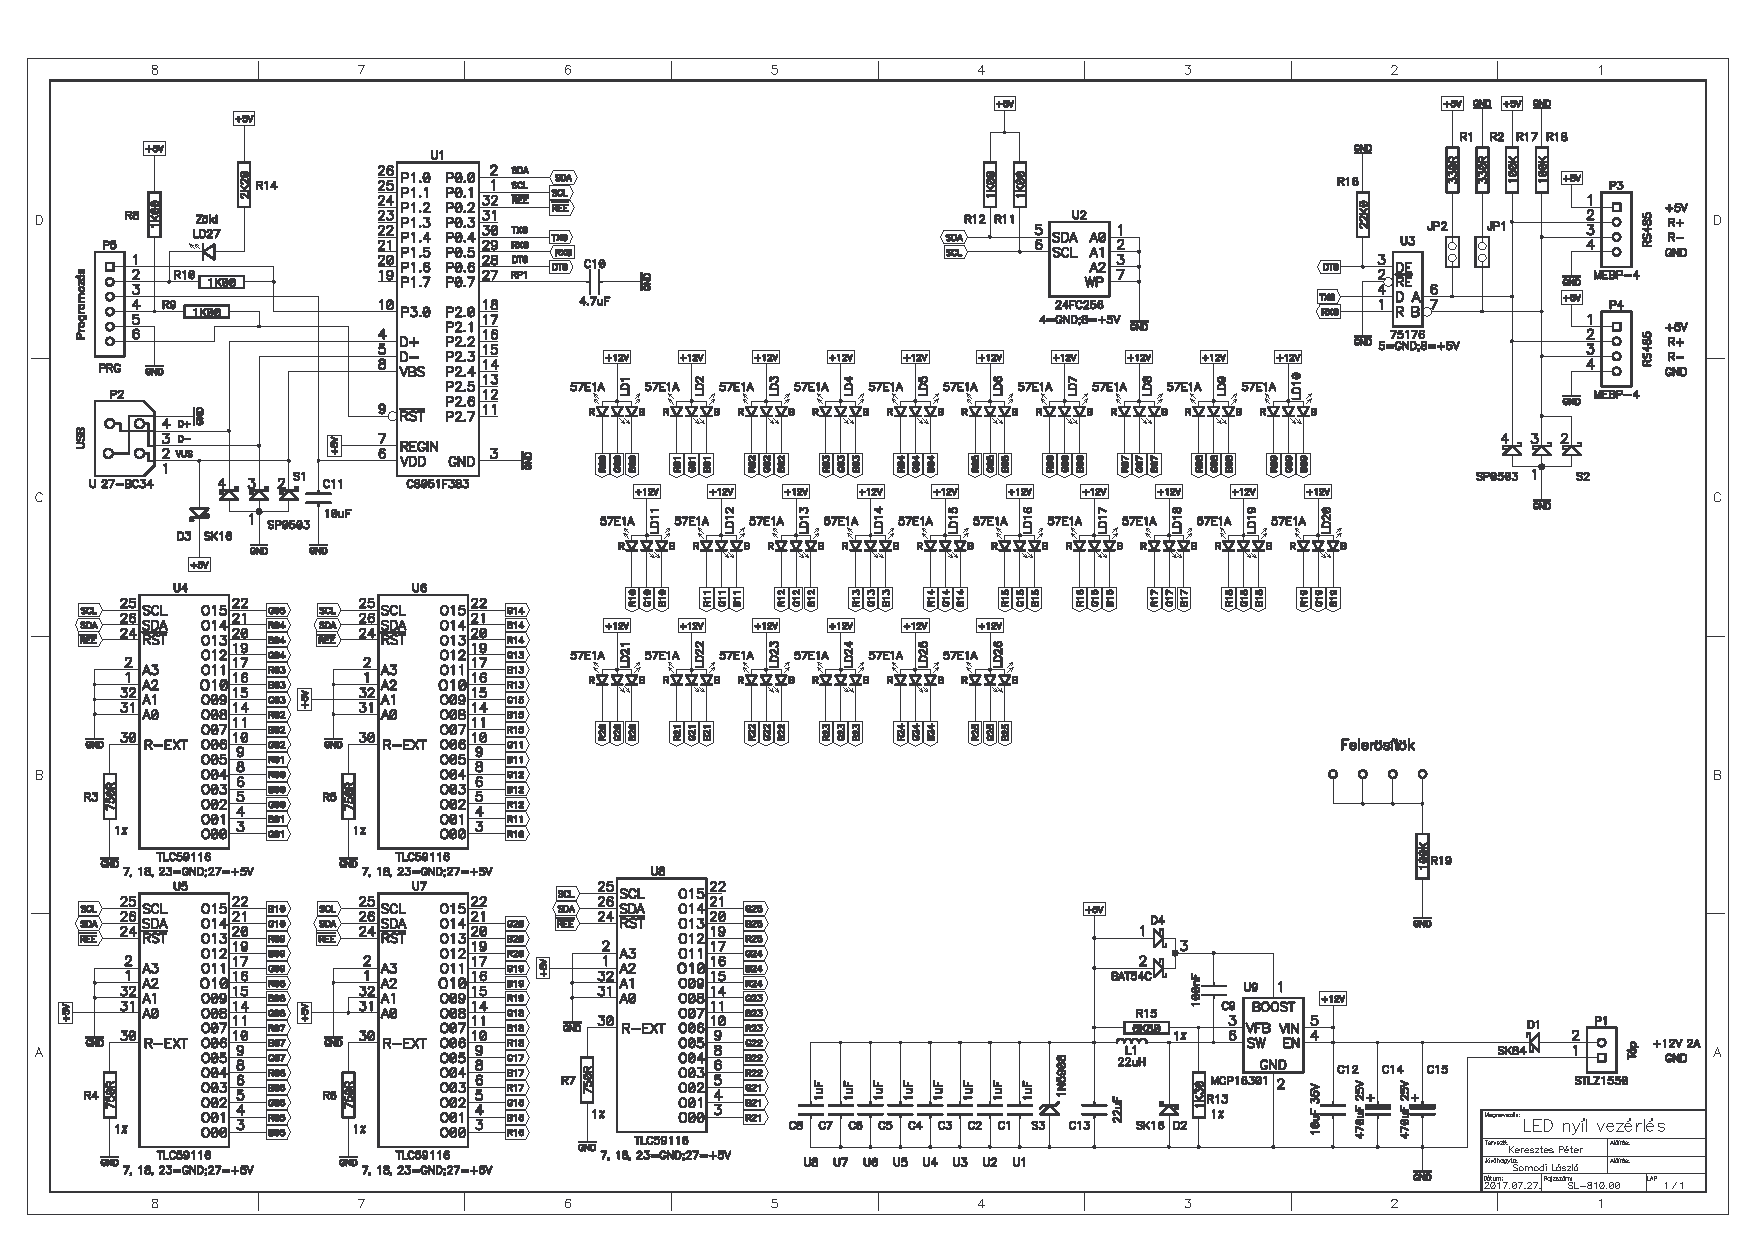
\includegraphics[page=1,width=0.5\textwidth]{SLN}
		
		\caption{nyíl kapcsolási rajz \#1}
		\label{fig:nyil1}
	\end{figure}
	\begin{figure}[h]
		\centering
		\includegraphics[page=2,width=0.5\textwidth]{SLN}
		
		\caption{nyíl kapcsolási rajz \#2}
		\label{fig:nyil2}
	\end{figure}
	\begin{figure}[h]
		\centering
		\includegraphics[page=3,width=0.5\textwidth]{SLN}
		
		\caption{nyíl kapcsolási rajz \#3}
		\label{fig:nyil3}
	\end{figure}




	\begin{comment}
		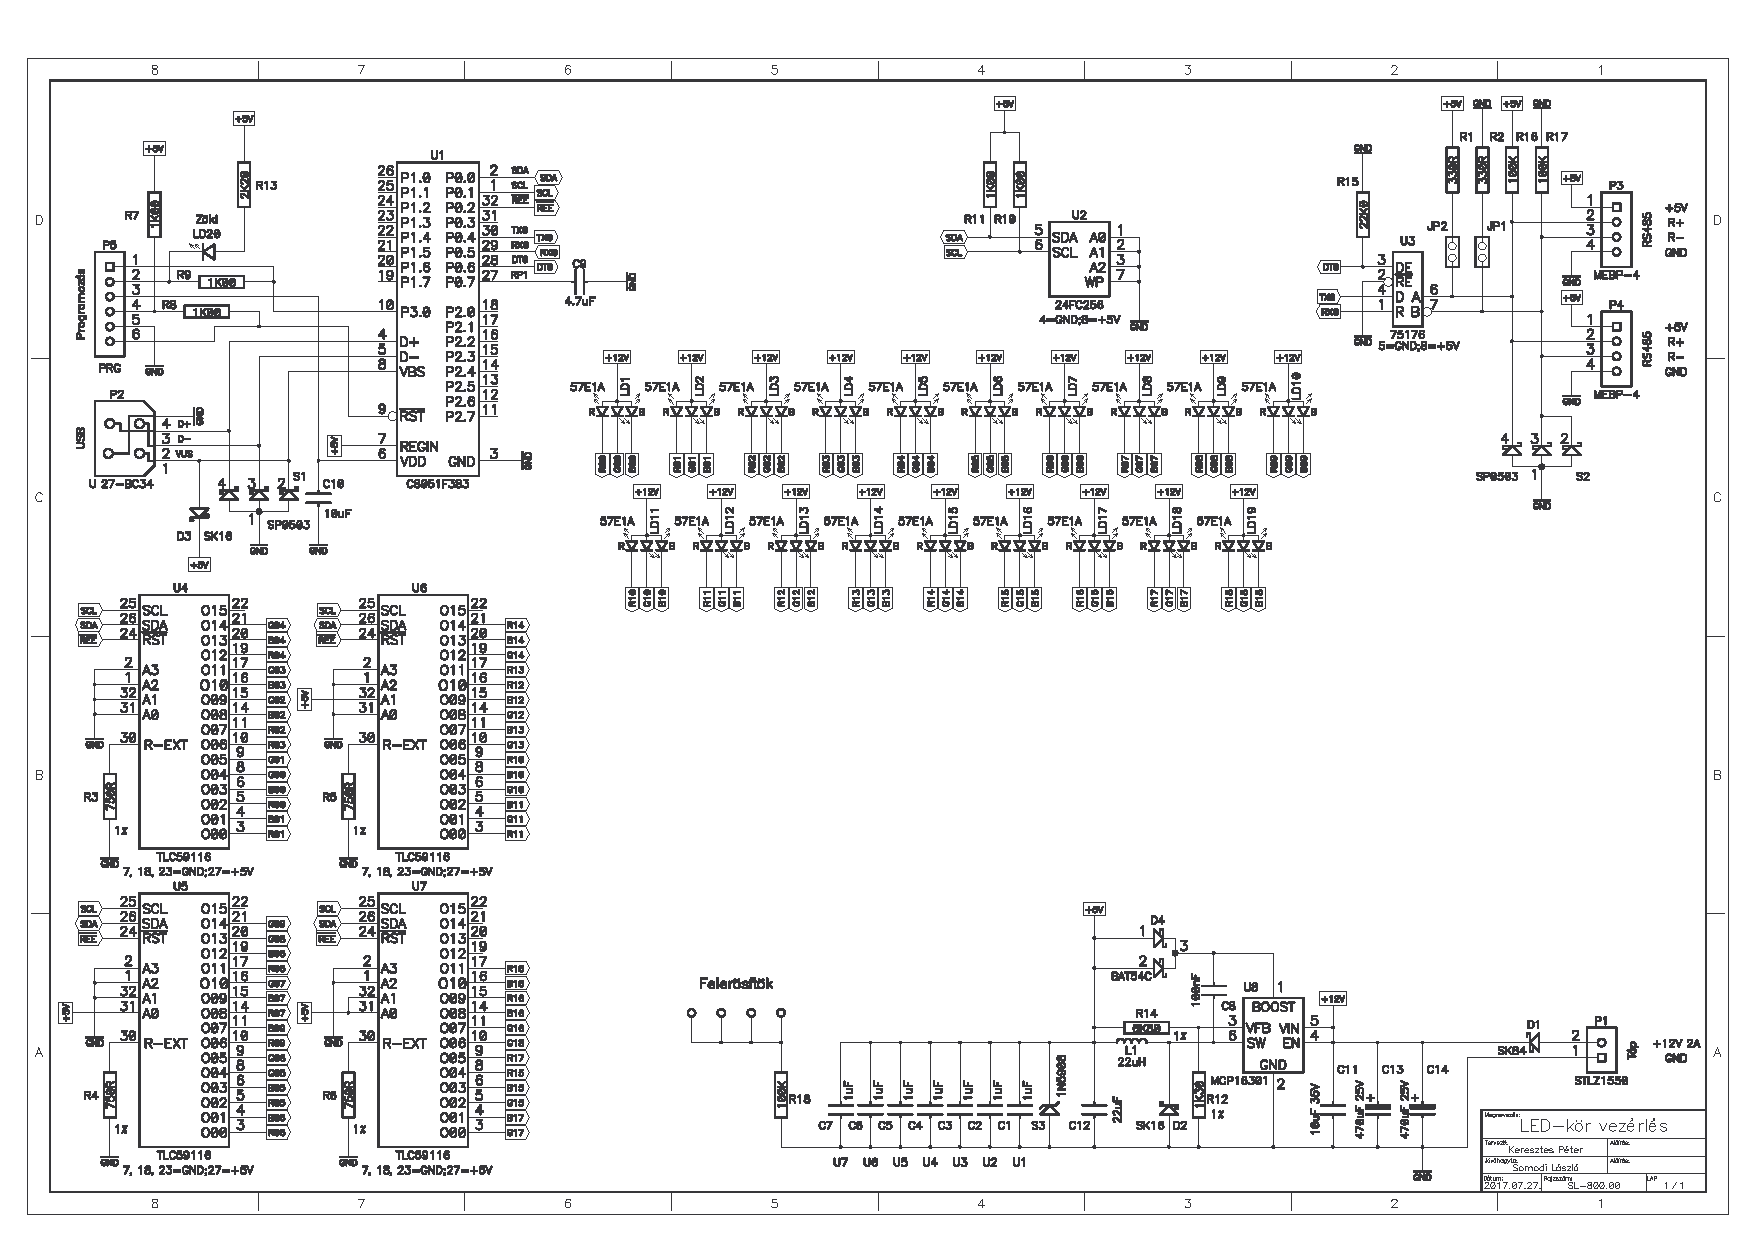
\includegraphics[width=0.5\textwidth]{SLL}
		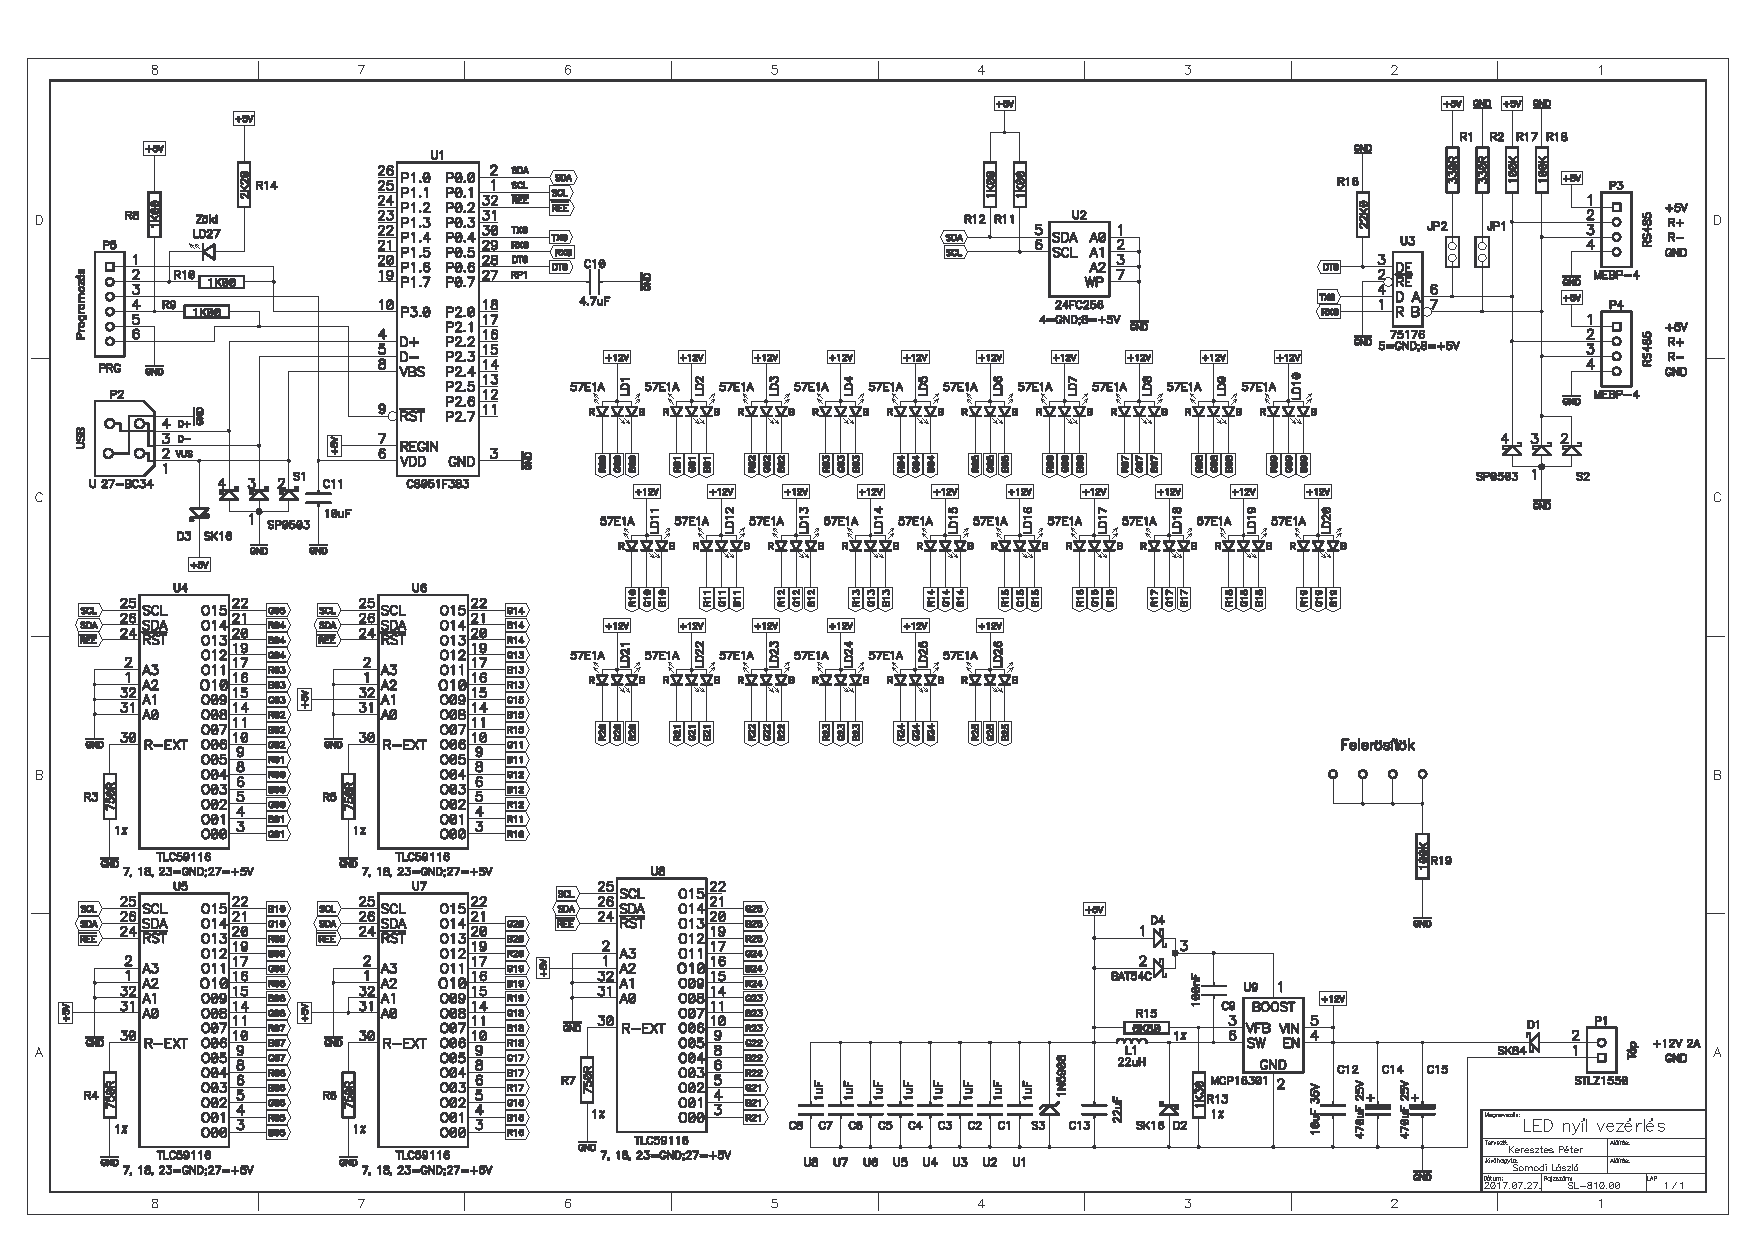
\includegraphics[width=0.5\textwidth]{SLN}
	\end{comment}
	\begin{comment}
		2.fejezet: Melyik részét csinálom én? Mit csináltunk, és hogyan ui-t kellett fejleszteni, milyen lépésekből állt, képernyőképekkel, eladjuk a munkánkat.
	\end{comment}
	\begin{comment}
		2.fejezet: Melyik részét csinálom én? Mit csináltunk, és hogyan ui-t kellett fejleszteni, milyen lépésekből állt, képernyőképekkel.
	\end{comment}
	\chapter*{2.fejezet}
	A jelenlegi fejezetben magáról a kódról és a felhasználó élményről szeretnék beszélni.
	A korábbi fejezetekben már említést tettem azon kapcsán, hogy az alkalmazást a C\# programozási nyelvben írom. Ezenfelül, egy olyan asztali alkalmazást szerettem volna készíteni amely apelláló lehet a felhasználó számára. Továbbá, a megjelenéstől, és a küllemtől eltekintve fontosnak tartom azt is, hogy egyszerű legyen az alkalmazás használata.
	\\
	A felületnek fontos jellemzője, hogy reszponzív legyen. Amikor a "reszponzív" kifejezést használjuk akkor a "reszponzív kinézetet" értjük. Ez azt jelenti, hogy az adott alkalmazás elérhető és alkalmazkodó legyen mindenféle eszközön. Akár itt értjük azokat az eszközöket amelyeknél nincsen kifejezetten sok beépített periféria, ilyenek például a okostelefon, tablet. Az ilyen eszközök során, fontos azt megoldani, hogy az alkalmazásban lévő objektumok(gombok, címkék) könnyen észlelhető, és elérhető lehessen a felhasználó számára. 
	\begin{comment}
		3.fejezet(vége): kitekintés, milyen más rendszerek vannak még, és ahhoz képest ez mit tud, vannak hasonló szoftverek, vannak tréner szoftverek, de a mienk az spec képzésre alkalmas
		- szoftver és a hardvert hozzákellett fejleszteni, ez egy prototípus.
	\end{comment}
	\chapter*{3.fejezet}
	\begin{comment}
		4.fejezet: (future works) továbbiakban milyen kimenetele lesz, ebből szabadalom lesz, az ötletgazda szeretné ezt kiadni olyan módon hogy piaci termék legyen. 
		- Teljesen más technológia
	\end{comment}
	\chapter*{4.fejezet}
	\begin{comment}
		5.fejezet:  összefoglaló, melyik fejezetben miről beszéltünk, miket sikerült elérni(pl 1.fejezetben említetteket megcsináltam, iylenek), Mi az EREDMÉNY! miért fontos, 
		- miért jó ez? Működés közben videókat kéne csinálni. Érdemes lenne titkosítani.
	\end{comment}
	\chapter*{Összegzés}
	


	
	\verb*|#TODO|: Összefoglalás...
	\bibliographystyle{plain}
	\bibliography{references}
	\begin{comment}
		1.Alapötlet, Projekt célja, és hatásai az oktatásra/egézségügyre.
				Miért jó a projekt amit csinálunk?
				Somodi László által kapottak megemlítése
		2.A Winformos projekt
				milyen eszközöket lehet irányítani vele(mire jók)
				panelek külön-külön mit csinálnak
				hogyan kommunikál a Delphi-vel (Bence projektje, megemlítés)
		3. Alacsonyabbszintű komponensek/Imperatív és oop közti kommunikáció(Bence)
				Hangvezérlés
				Színek
				Nyilak
				4 || 8 eszközös megoldások
		4. Projekt tényleges használata, felmérések, és vélemények.
				Gondolatok és meglátások //akár lehet egyel előbb is
	\end{comment}
	% Aláírt, szkennelt nyilatkozat beillesztése a szakdolgozat végére
	%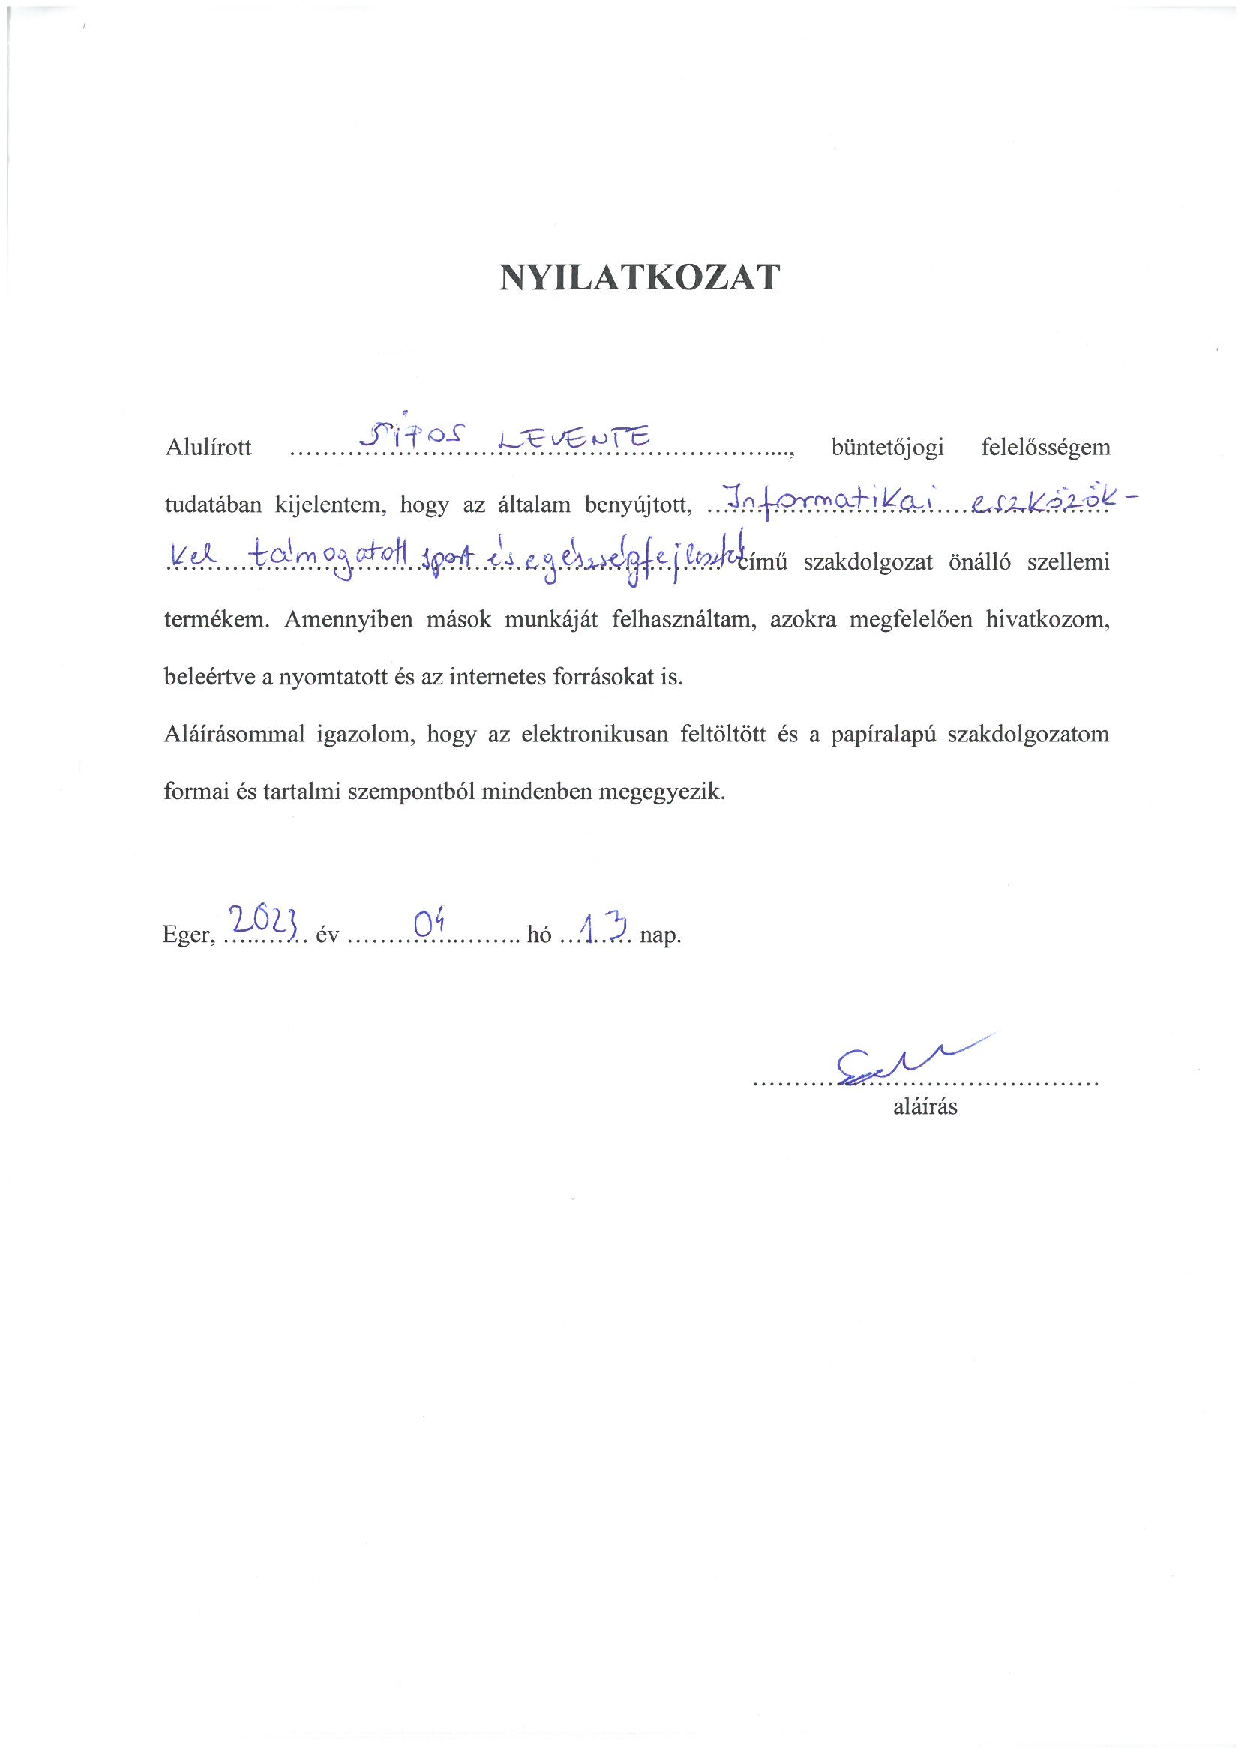
\includepdf{nyilatkozat.pdf}
		\listoffigures
\end{document}